\documentclass[a4paper,12pt]{article}
\usepackage[a4paper,top=1.3cm,bottom=2cm,left=1.5cm,right=1.5cm,marginparwidth=0.75cm]{geometry}
\usepackage{cmap}
\usepackage{mathtext}
\usepackage[T2A]{fontenc}
\usepackage[utf8]{inputenc}
\usepackage[english,russian]{babel}
\usepackage{siunitx}
\usepackage{enumitem}
\usepackage{placeins}

\usepackage{graphicx}

\usepackage{wrapfig}
\usepackage{tabularx}
\usepackage{multirow}

\usepackage{hyperref}
\usepackage[rgb]{xcolor}
\hypersetup{
colorlinks=true,urlcolor=blue
}
\usepackage{amsmath,amsfonts,amssymb,amsthm,mathtools}
\usepackage{icomma}
\mathtoolsset{showonlyrefs=false}
\usepackage{euscript}
\usepackage{mathrsfs}
\DeclareMathOperator{\sgn}{\mathop{sgn}}
\newcommand*{\hm}[1]{#1\nobreak\discretionary{}
{\hbox{$\mathsurround=0pt #1$}}{}}

%%% Заголовок
\author{Макаров Лев Евгеньевич}
\title{Лабораторная работа №3.5.1

Изучение плазмы газового разряда в неоне
}
\date{\today}

\begin{document}

\begin{titlepage}
	\begin{center}
		{\large МОСКОВСКИЙ ФИЗИКО-ТЕХНИЧЕСКИЙ ИНСТИТУТ (НАЦИОНАЛЬНЫЙ ИССЛЕДОВАТЕЛЬСКИЙ УНИВЕРСИТЕТ)}
	\end{center}
	\begin{center}
		{\large Физтех-школа фотоники, электроники и молекулярной физики}
	\end{center}
	
	
	\vspace{4.5cm}
	{\huge
		\begin{center}
			{\bf Отчёт о выполнении лабораторной работы 4.3.2}\\
			Дифракция света на ультрозвуковой волне в жидкости
		\end{center}
	}
	\vspace{2cm}
	\begin{flushright}
		{\LARGE Автор:\\ Макаров Лев Евгеньевич \\
			\vspace{0.2cm}
			Б04-306}
	\end{flushright}
	\vspace{8cm}
	\begin{center}
		Долгопрудный 2025
	\end{center}
\end{titlepage}

\section{Введение}

\textbf{Цель работы:} 
\begin{enumerate}
	\item Изучение дифракции света на синусоидальной акустической решётке и наблюдение фазовой решётки методом тёмного поля
\end{enumerate}

\textbf{В работе используются:} 
\begin{itemize}
    \item оптическая скамья
    \item осветитель
    \item два длиннофокусных объектива
    \item кювета с жидкостью
    \item кварцевый излучатель с микрометрическим винтом
    \item генератор ультразвуковой частоты
    \item линза
    \item вертикальная нить на рейтере
    \item микроскоп
\end{itemize}
\medskip

\section{Теоретические сведения}

В работе используются оптическая скамья, осветитель, два длиннофокусных объектива, кювета с жидкостью, кварцевый излучатель с микрометрическим винтом, генератор звуковой частоты, линза, горизонтальная нить на рейтере, микроскоп. 
	
При прохождении ультразвуковой волны через жидкость в ней возникают периодические неоднородности коэффициента преломления, создается фазовая решетка, которую мы считаем неподвижной ввиду малости скорости звука относительно скорости света. Показатель
преломления n изменяется по закону:

\begin{equation}\label{}
    n = n_0 (1 + m \cos \Omega x)
\end{equation}

Здесь $ \Omega = 2 \pi / \Lambda $ --- волновое число для ультразвуковой волны, $ m $ --- глубина модуляции $ n $ $ (m \ll 1 $).

Положим фазу $ \phi $ колебаний световой волны на передней стенке кюветы равной нулю, тогда на задней поверхности она равна:

\begin{equation}\label{}
    \phi  = k n L = \phi_0 (1 + m \cos \Omega x)
\end{equation}

Здесь $ L $ --- толщина жидкости в кювете, $ k = 2 \pi / \lambda $ --- волновое число для света.

После прохождения через кювету световое поле есть совокупность плоских волн, распространяющихся под углами $ \theta $, соответствующими максимумам в дифракции Фраунгофера:

\begin{equation}\label{}	
    \Lambda \sin \theta_m = m \lambda
\end{equation}

Этот эффект проиллюстрирован на рис. \ref{pic:difraction}.
\begin{figure}[h!]
    \centering	
    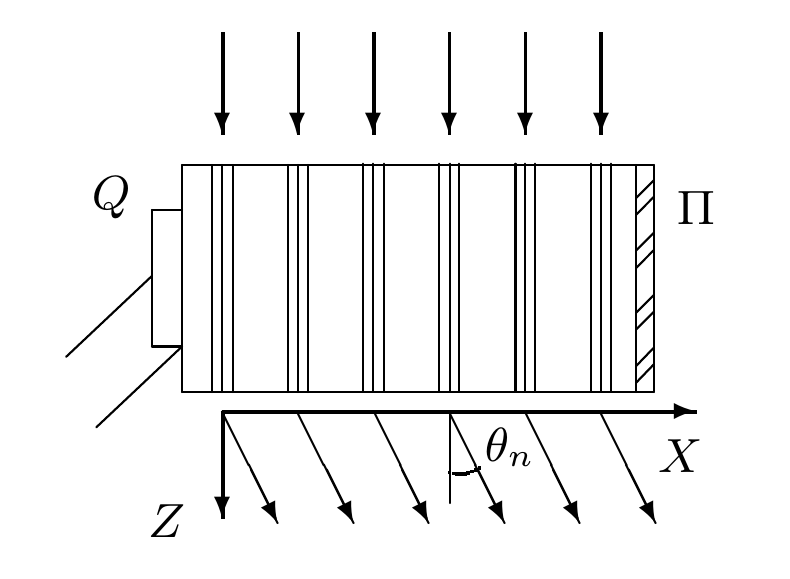
\includegraphics[width=0.3\textwidth]{images/difraction.png}
    \caption{Дифракция световых волн на акустической решетке}
    \label{pic:difraction}
\end{figure}

Зная положение дифракционных максимумов, по формуле (1) легко определить длину ультразвуковой волны, учитывая малость $ \theta $: $ \sin \theta \approx \theta \approx l_m /F  $, где $ l_m $ --- расстояние от нулевого до последнего видимого максимума, $ F $ --- фокусное расстояние линзы. Тогда получим:

\begin{equation}\label{}
 \Lambda = m \lambda F/ l_m 
\end{equation}
Скорость ультразвуковых волн в жидкости, где $ \nu $ --- частота колебаний излучателя:

\begin{equation}\label{}
	v = \Lambda \nu 
\end{equation}

\section{Экспериментальная установка}

Схема установки представлена на рис. \ref{pic:ustan}. Источник света Л с помощью конденсора К проецируется на входную щель $S$. Входная щель ориентирована горизонтально и прикрыта красным светофильтром Ф. Коллиматорный объектив $\text{О}_1$ посылает параллельный пучок на кювету с водой $С$. Излучатель Q создаёт УЗ-волну. Параллельный пучок света, дифрагируя на стоячей звуковой волне, образует дифракционную картину в фокальной плоскости $F$ камерного объектива $\text{О}_{2}$. Картину можно наблюдать в микроскоп М.

\FloatBarrier
\begin{figure}[!h]
	\centering
	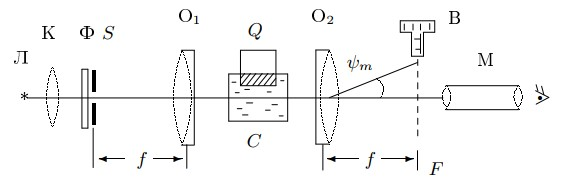
\includegraphics[width=0.6\linewidth]{images/ustan.jpg}
	\caption{Схема установки для наблюдения дифракции на акустической фазовой решетке}
	\label{pic:ustan}
\end{figure}
\FloatBarrier



\FloatBarrier
\begin{figure}[h]
    \begin{minipage}[h]{0.5\linewidth}
        \center{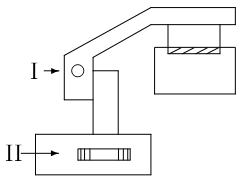
\includegraphics[width=0.6\linewidth]{images/vertical-move-ustan.png}}
        \caption{Устройство для вертикального перемещения излучателя}
        \label{pic:vertical-move-ustan}
    \end{minipage}
    \begin{minipage}[h]{0.5\linewidth}
        \center{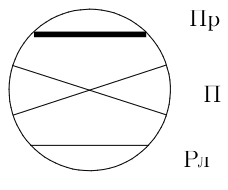
\includegraphics[width=0.6\linewidth]{images/cross.png}}
        \caption{Проволока Пр, перекрестие П и реперная линия Рл в фокальной плоскости объектива $O_2$}
        \label{pic:cross}
    \end{minipage}
\end{figure}
\FloatBarrier

Дифракционные полосы ориентированы горизонтально. Расстояние между ними можно измерить с помощью микрометрического винта B.


Длина $\Lambda$ ультразвуковой волны определяется с помощью уравнения \eqref{eq:length}:

\begin{equation}\label{eq:length}
    \Lambda \sin{\theta_m} = m \lambda
\end{equation}

Так как углы $\theta_m$ малые, то окончательное выражение можно упростить:

\begin{equation}\label{eq:final}
    l_m = m f \frac{\lambda}{\Lambda}
\end{equation}

где $l_m$ -- измеренное на опыте линейное расстояние между $m$-м и нулевым максимумами, а $f$ -- фокусное расстояние объектива $O_2$.

Скорость распространения звука в воде можно рассчитать по формуле:

\begin{equation}\label{eq:sound-speed}
    v = \Lambda \nu
\end{equation}

если известна частота $\nu$ кварцевого излучателя

\subsection*{Метод темного поля}

Схема установки для данного метода приведена на рис. \ref{pic:dark-field}.

С помощью вспомогательной линзы O, расположенной на оптической скамье за фокальной плоскостью объектива $\text{O}_2$ можно получить изображение задней плоскости. Перемещая микроскоп вдоль оптической оси, фокусируем его на плоскость P, где расположено четкое изображение $a'b'$ какого-либо предмета $ab$, вплотную прижатого к стенке кюветы.

\FloatBarrier
\begin{figure}[!h]
	\centering
	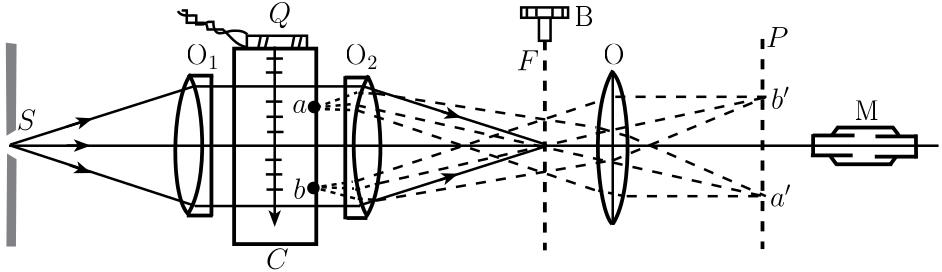
\includegraphics[width=0.6\linewidth]{images/dark-field.png}
	\caption{Наблюдение акустической решетки методом тёмного поля}
	\label{pic:dark-field}
\end{figure}
\FloatBarrier

Метод тёмного поля основан на устранении центрального максимума с помощью специального экрана (перекрывается проволокой). В поле зрения микроскопа наблюдаются темные и светлые полосы. Расстояние между тёмными соответствует смещению в плоскости кюветы на $\Lambda/2$.


\section{Результаты измерений и обработка данных}

\begin{enumerate}
    \item Соберем схему установки согласно рис. \ref{pic:ustan}. Максимально откроем входную щель. Поместив лист бумаги между коллиматором и кюветой, убедимся, что она равномерно освещается. Проверим так же свет на выходе из прибора. Настроим микроскоп, отсчётное устройство и установим рабочую ширину щели 20 мкм.
    \item Получим в поле зрения микроскопа дифракционную картину
\end{enumerate}

Перемещая излучатель, оценим длину УЗ волны как удвоенное расстояние между наиболее четкими дифракционными картинами: $2 \Lambda = 140 \cdot 10$ мкм. Подставим в уравнение \eqref{eq:sound-speed}, где частота кварцевого излучателя $\nu = 2,17$ МГц.

\begin{equation*}
    v = \Lambda \nu = 70 \cdot 10 \cdot 2,17 \approx 1519 \ \text{м/с}
\end{equation*}

\begin{enumerate}[resume]
    \item определим положение дифракционных полос.
\end{enumerate}

Подберем частоту генератора, при которой видна дифракционная картина $\nu = 2,17$ МГц. Вращением лимба добьемся наилучшей картины, чтобы было видно максимальное число полос.

С помощью перекрестия и микрометрического винта определим координату Y каждой видной полосы. Результаты измерений запишем в таблицу \ref{table:1}.

\FloatBarrier
\begin{table}[!h]
    \centering
    \caption{\textit{Измерение положения полос при разных частотах}}
    \begin{tabular}{|l|llllllllll|}
    \hline
                     & \multicolumn{10}{l|}{положения, 1 дел = 4 мкм} \\ \hline
        $\nu$, Мгц & \multicolumn{1}{l|}{1}   & \multicolumn{1}{l|}{2}   & \multicolumn{1}{l|}{3}   & \multicolumn{1}{l|}{4}   & \multicolumn{1}{l|}{5}   & \multicolumn{1}{l|}{6}   & \multicolumn{1}{l|}{7}   & \multicolumn{1}{l|}{8}   & \multicolumn{1}{l|}{9}   & 10  \\ \hline
        2,17         & \multicolumn{1}{l|}{50}  & \multicolumn{1}{l|}{34}  & \multicolumn{1}{l|}{16}  & \multicolumn{1}{l|}{3}   & \multicolumn{1}{l|}{-13} & \multicolumn{1}{l|}{-32} & \multicolumn{1}{l|}{-51} & \multicolumn{1}{l|}{-65} & \multicolumn{1}{l|}{-89} & -95 \\ \hline
        3,2          & \multicolumn{1}{l|}{}    & \multicolumn{1}{l|}{}    & \multicolumn{1}{l|}{24}  & \multicolumn{1}{l|}{13}  & \multicolumn{1}{l|}{-20} & \multicolumn{1}{l|}{-40} & \multicolumn{1}{l|}{-77} & \multicolumn{1}{l|}{-98} & \multicolumn{1}{l|}{}    &     \\ \hline
        1,93         & \multicolumn{1}{l|}{135} & \multicolumn{1}{l|}{121} & \multicolumn{1}{l|}{107} & \multicolumn{1}{l|}{93}  & \multicolumn{1}{l|}{80}  & \multicolumn{1}{l|}{64}  & \multicolumn{1}{l|}{42}  & \multicolumn{1}{l|}{30}  & \multicolumn{1}{l|}{20}  & 6   \\ \hline
        4,1          & \multicolumn{1}{l|}{}    & \multicolumn{1}{l|}{}    & \multicolumn{1}{l|}{138} & \multicolumn{1}{l|}{123} & \multicolumn{1}{l|}{82}  & \multicolumn{1}{l|}{61}  & \multicolumn{1}{l|}{18}  & \multicolumn{1}{l|}{0}   & \multicolumn{1}{l|}{}    &     \\ \hline
        2,7          & \multicolumn{1}{l|}{}    & \multicolumn{1}{l|}{}    & \multicolumn{1}{l|}{117} & \multicolumn{1}{l|}{104} & \multicolumn{1}{l|}{81}  & \multicolumn{1}{l|}{61}  & \multicolumn{1}{l|}{31}  & \multicolumn{1}{l|}{17}  & \multicolumn{1}{l|}{}    &     \\ \hline
    \end{tabular}
    \label{table:1}
\end{table}


\begin{enumerate}[resume]
    \item Повторим измерения предыдущего пункта для других частот, рещультаты измерений запишем в таблицу \ref{table:1}. Отключим генератор.
    \item Закроем проволочкой центральный максимум и запишем показания винта: 622 дел.
    \item Построим графики зависимости $Y = Y(m)$ для каждой частоты.
\end{enumerate}

\FloatBarrier
\begin{figure}[!ht]
        \centering
	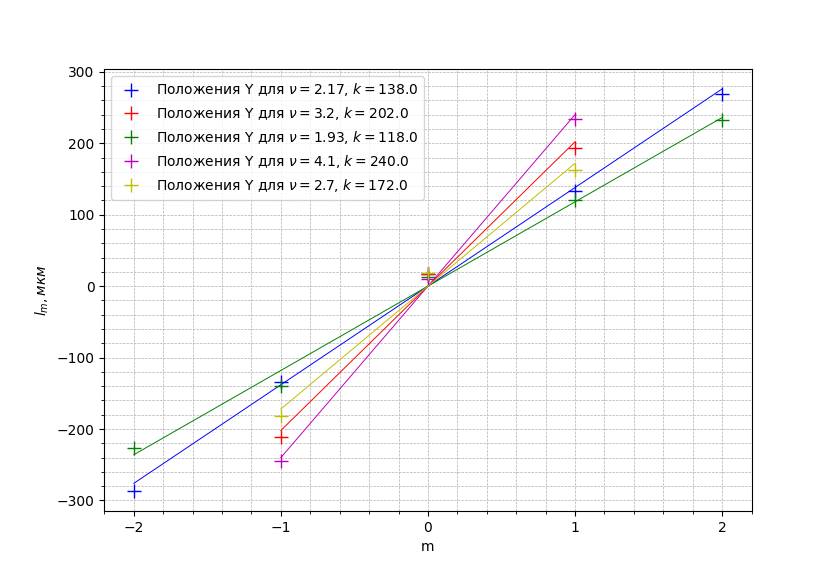
\includegraphics[width=1.0\textwidth]{images/graph-1.png}
	\caption{\textit{Зависимости $Y = Y(m)$}}
	\label{graph:1}
\end{figure}
\FloatBarrier

\clearpage

Имея формулы \eqref{eq:final} получаем:

\begin{equation*}
    l_m = m f \frac{\lambda}{\Lambda} = k m \ \implies \ k = f \frac{\lambda}{\Lambda} \ \implies \ \Lambda = f \frac{\lambda}{k}
\end{equation*}

Посчитаем $\Lambda$ для каждой частоты и запишем в таблицу \ref{table:2}. Для каждой частоты посчитаем скорость звука и запишем в таблицу \ref{table:2}.

\begin{table}[!ht]
    \centering
    \caption{\textit{Вычисление $\Lambda$ и $v$ для каждой частоты}}
    \begin{tabular}{|l|l|l|l|l|l|l|l|}
        \hline
        $\nu$, Мгц & $\sigma_\nu$, МГц & $k$, мкм & $\sigma_k$, мкм & $\Lambda$, мм & $\sigma_\Lambda$, мм & $v$, м/с & $\sigma_v$, м/с \\ \hline
        2,17 & 0,05 & 138 & 3 & 1,30 & 0,05 & 1400   & 100  \\ \hline
        3,20 & 0,05 & 202 & 9 & 0,89 & 0,05 & 1400   & 100  \\ \hline
        1,93 & 0,05 & 118 & 4 & 1,52 & 0,08 & 1450   & 100  \\ \hline
        4,10 & 0,05 & 240 & 5 & 0,75 & 0,03 & 1550   & 100  \\ \hline
        2,70 & 0,05 & 172 & 9 & 1,04 & 0,07 & 1400   & 100  \\ \hline
    \end{tabular}
    \label{table:2}
\end{table}

\begin{enumerate}[resume]
    \item Посчитаем все погрешности. Результаты по порядку величины совпадают с теоритическими.
\end{enumerate}

Дальнейшие пункты работы не выполнялись.



\end{document}